% Chapter 3

\chapter{Estrutura do Gimbal} % Main chapter title
\label{chap:Chapter5} % For referencing the chapter elsewhere, use \ref{chap:Chapter3} 

%----------------------------------------------------------------------------------------


A conceção do \emph{gimbal} foi realizada de raiz utilizando o \emph{software} \emph{Blender}, priorizando a rigidez estrutural e a funcionalidade modular. Para o eixo de \emph{pitch}, optou-se por uma configuração de apoio duplo, garantindo que a carga útil seja sustentada em ambas as extremidades. Esta arquitetura dissipa as solicitações mecânicas pelos suportes laterais, evitando a aplicação de cargas radiais () diretamente no veio do motor, o que previne a sua degradação precoce e assegura a repetibilidade do posicionamento. Relativamente ao eixo de \emph{yaw}, utilizou-se uma configuração de apoio simples, visto que a carga está alinhada com o centro de gravidade do sistema, resultando numa componente de carga predominantemente axial sobre o motor. Esta estrutura teve como inspiração o sistema HELIOS da Lockheed Martin, adotando princípios de desenho da referida plataforma de defesa.

A construção do protótipo recorreu à manufatura aditiva por FDM (\emph{Fused Deposition Modeling}) numa impressora Creality Ender 3 SE, utilizando o polímero PLA (\emph{Polylactic Acid}). Este material foi selecionado pelo compromisso ideal entre facilidade de prototipagem, rigidez mecânica e baixo custo. As principais configurações utilizadas para a manufatura foram compiladas na Tabela~\ref{tab:config_impressao3d}.

\begin{longtable}{ll}
    \caption[Configurações Principais da Impressão 3D]{Parâmetros e configurações detalhadas do processo de impressão 3D das componentes do sistema.} \label{tab:config_impressao3d} \\
    \toprule
    \textbf{Parâmetro / Configuração} & \textbf{Valor Definido} \\
    \midrule
    \endhead % Tudo o que estiver acima desta linha repete-se no topo da nova página, caso mude de página
    
    \bottomrule
    \endfoot % O que aparece no fundo de cada página enquanto a tabela não terminar
    
    Temperatura do Bico (1.ª Camada) & 205 °C \\
    Temperatura do Bico (Restantes Camadas) & 200 °C \\
    Temperatura da Mesa & 50 °C \\
    Multiplicador de Extrusão (\emph{Flow}) & 0.87 \\
    Altura da Camada & 0.12 mm \\
    Densidade de Preenchimento (\emph{Infill}) & 50\% \\
    Velocidade de Perímetros & 70 mm/s \\
    Velocidade de Preenchimento & 70 mm/s \\
    Velocidade de Preenchimento Sólido & 70 mm/s \\
    Velocidade de Deslocamento (\emph{Travel}) & 50 mm/s \\
    Aba (\emph{Brim}) & Ativada \\
\end{longtable}

A estrutura é composta por três módulos principais:
\begin{itemize}
    \item \textbf{Base:} O componente estacionário que serve de interface com a plataforma de suporte, onde se aloja o atuador responsável pelo movimento de \emph{yaw}.
    \item \textbf{Estrutura Central:} Esta peça atua como o elemento de ligação dinâmico; encontra-se acoplada ao eixo de \emph{yaw} e suporta, simultaneamente, o motor do eixo de \emph{pitch}. Esta configuração permite que a torre rode solidariamente com o movimento horizontal, transportando o sistema de elevação. Para facilitar a manutenção e montagem, a torre foi desenhada de forma tripartida, permitindo que os braços de suporte e o motor de \emph{pitch} sejam removidos de forma independente através de uniões aparafusadas.
    \item \textbf{Eixo de Pitch:} O componente final que contém a carga útil (o sistema laser e a câmara). Está acoplada ao motor de \emph{pitch} e, tal como mencionado anteriormente, beneficia de um apoio duplo.
\end{itemize}

Esta abordagem modular não só simplificou o processo de fabrico como permite a substituição rápida de componentes para iterações de design ou manutenção do sistema. O modelo montado apresenta uma altura de cerca de 13.6 cm e uma largura de cerca de 14 cm sendo está uma estrutura circular, assim como apresentado na figura:
\begin{figure}[H]
    \centering
    % Primeira Subfigura (Esquerda)
    \begin{subfigure}[b]{0.333\textwidth}
        \centering
        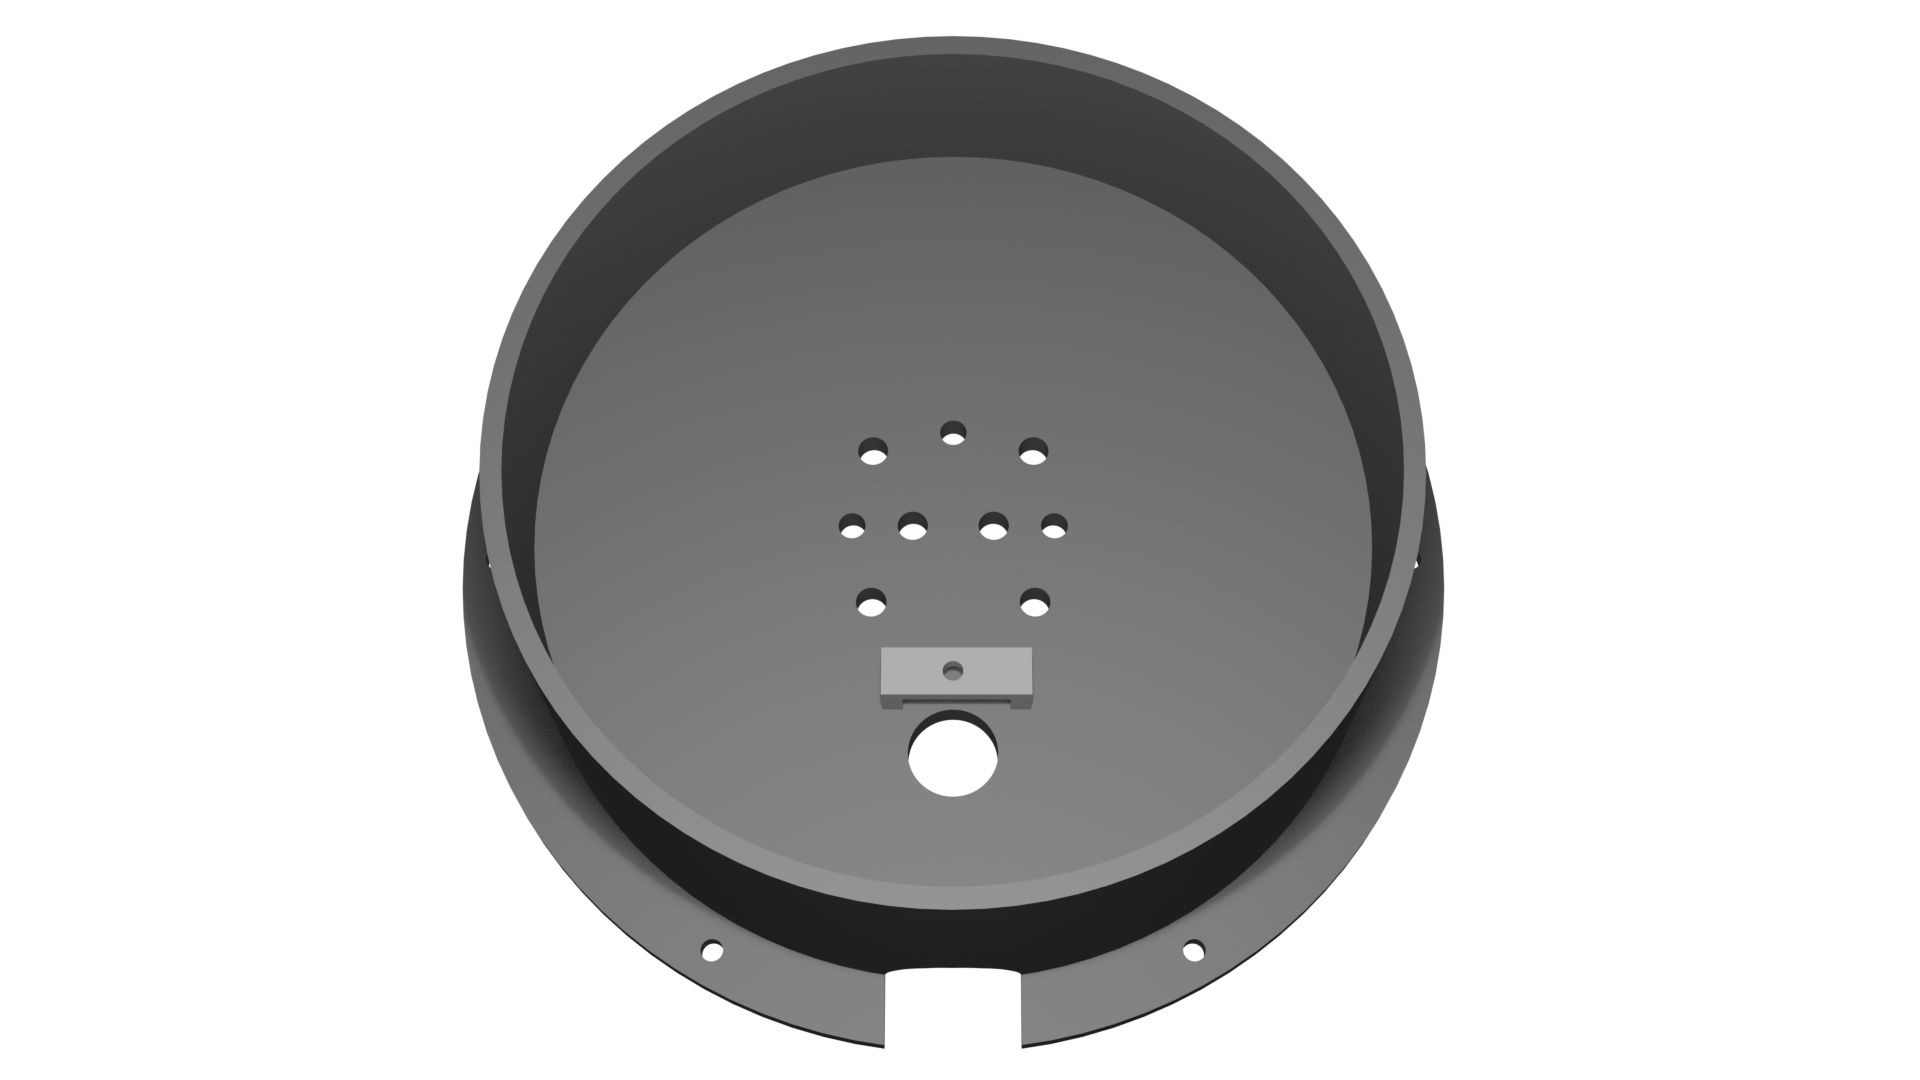
\includegraphics[width=\textwidth,keepaspectratio,trim={10cm 0 10cm 0},clip]{chapters/ch5_Estrutura/assets/base.png}
        \caption{Base.      }
        \label{fig:sub_base}
    \end{subfigure}\hfill
    % Segunda Subfigura (Centro)
    \begin{subfigure}[b]{0.333\textwidth}
        \centering
        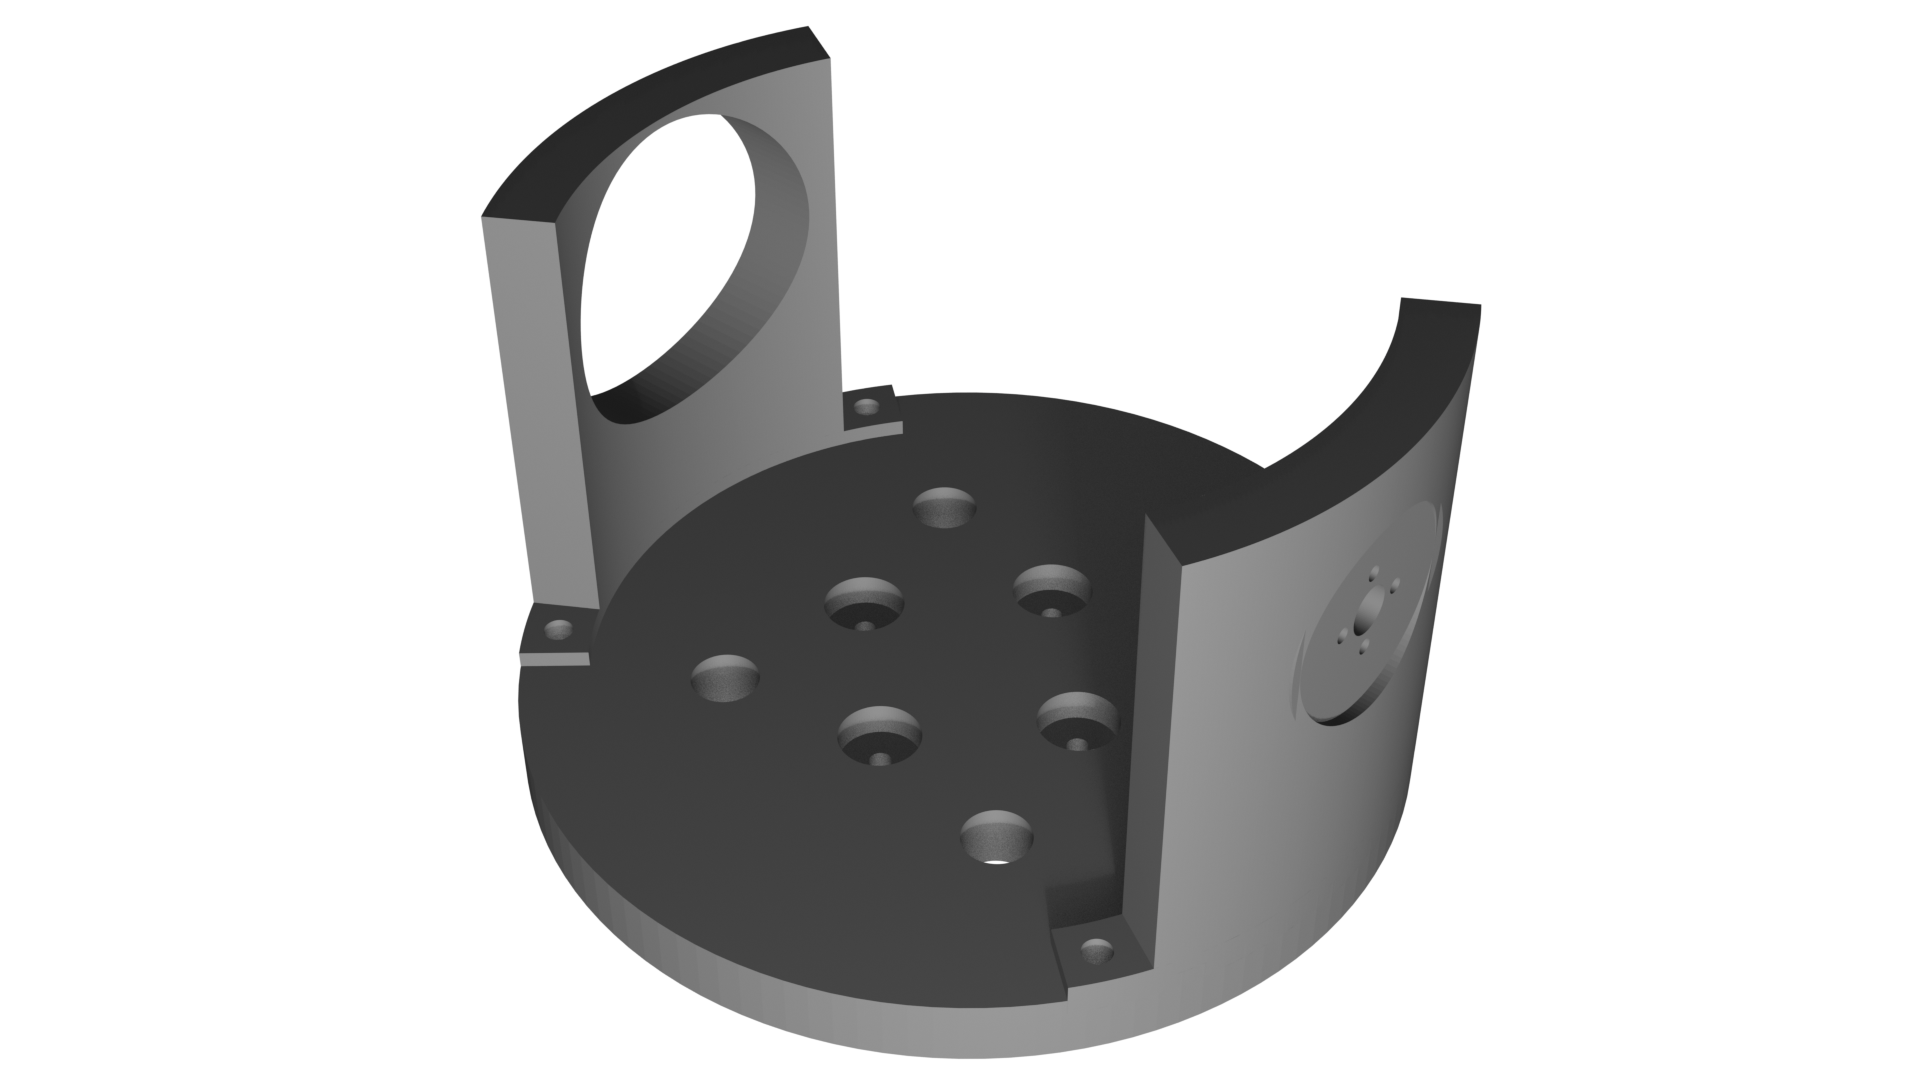
\includegraphics[width=\textwidth,keepaspectratio,trim={10cm 0 10cm 0},clip]{chapters/ch5_Estrutura/assets/torre_Yaw.png}
        \caption{Estrutura Central.}
        \label{fig:sub_braco}
    \end{subfigure}\hfill
    % Terceira Subfigura (Direita)
    \begin{subfigure}[b]{0.333\textwidth}
        \centering
        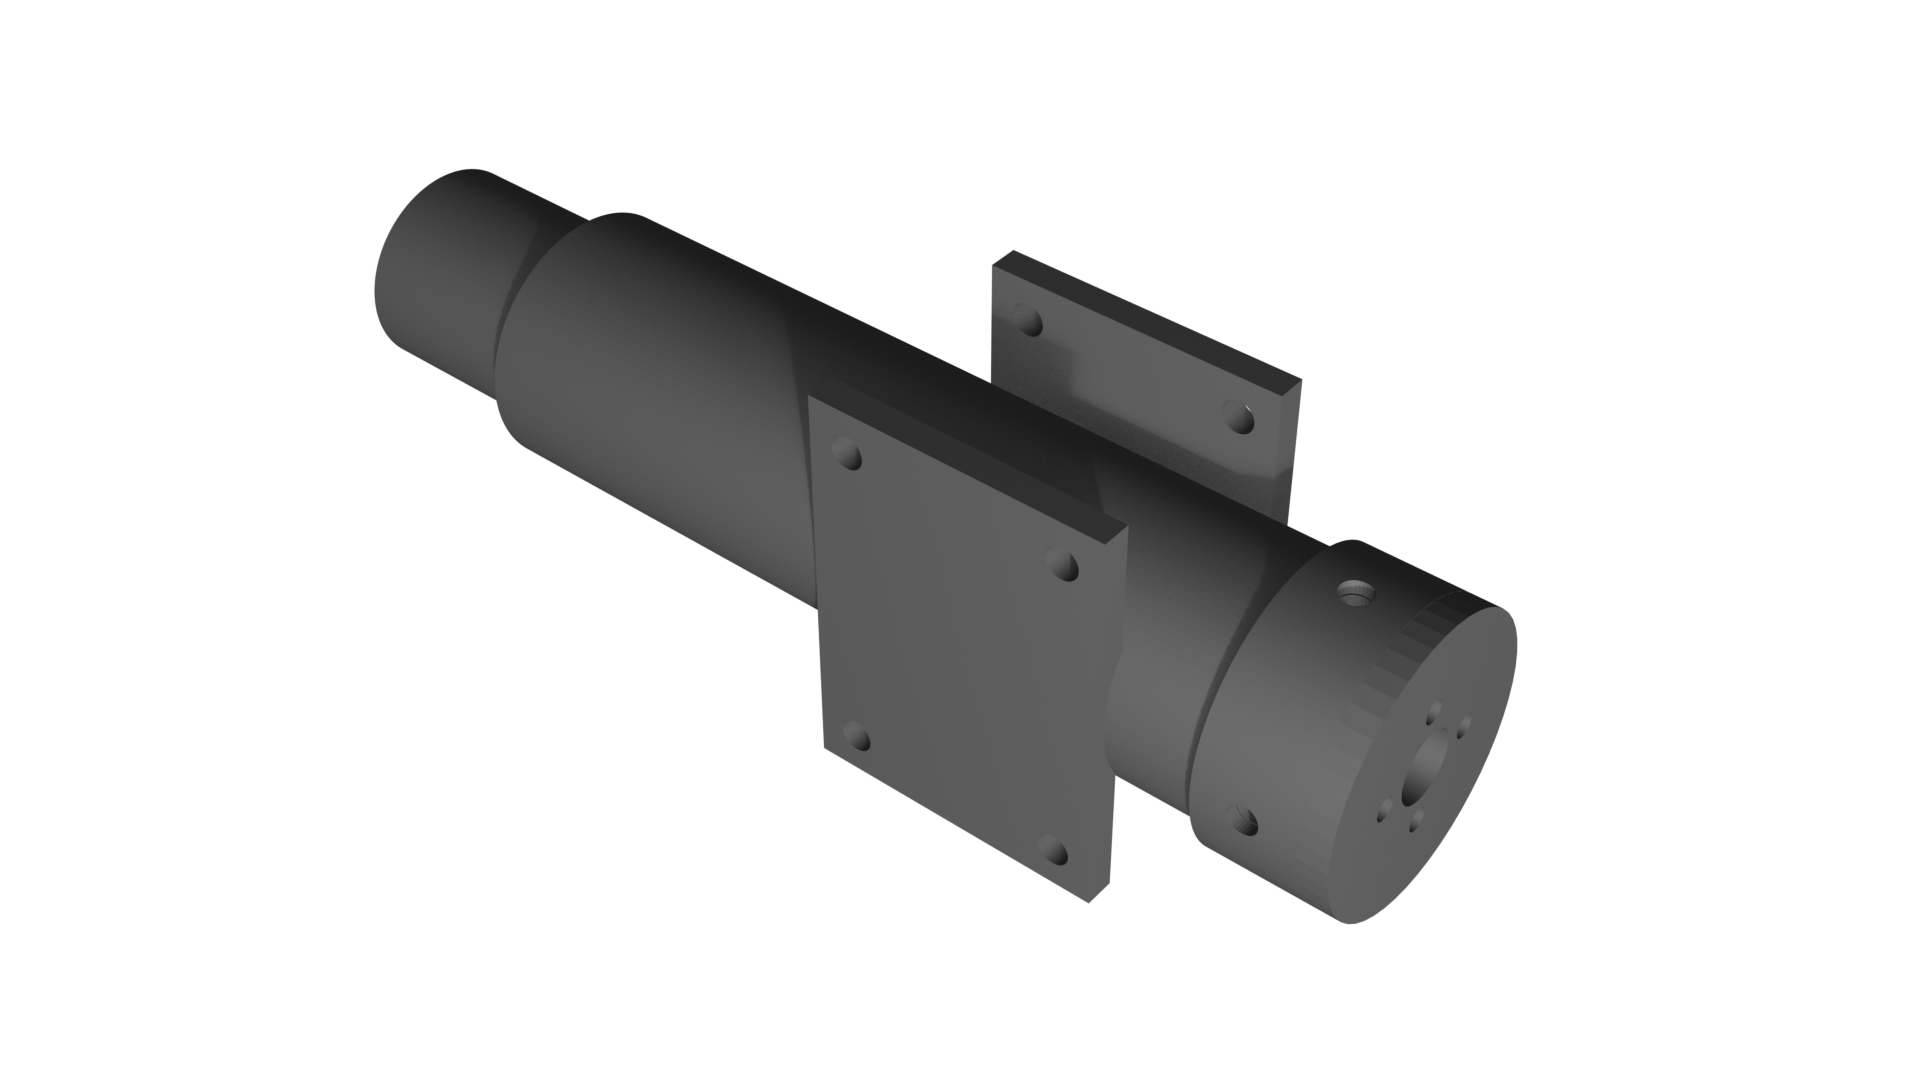
\includegraphics[width=\textwidth,keepaspectratio,trim={10cm 0 10cm 0},clip]{chapters/ch5_Estrutura/assets/eixo.png}
        \caption{Eixo de Pitch.}
        \label{fig:sub_pitch}
    \end{subfigure}
    
    % Legenda Geral da Figura Tripla
    \caption[Componentes Estruturais do Gimbal]{Representação tridimensional dos três módulos principais que constituem a estrutura do \emph{gimbal}.}
    \label{fig:componentes_gimbal}
\end{figure}


No total, a estrutura é composta por 7 peças impressas, distribuídas em 1 peça na base, 4 peças para a constituição da estrutura central e 2 peças para o eixo de \emph{pitch}. Na base, o componente corresponde ao próprio modelo. Na estrutura central, existe a peça de acoplamento ao motor de \emph{yaw} (fixo na base), a base da estrutura central e duas estruturas verticais responsáveis por suportar o motor e o rolamento de apoio do eixo de \emph{pitch}. No eixo de \emph{pitch}, existe uma peça encarregue da junção mecânica entre o corpo do eixo e o respetivo motor de elevação e o próprio eixo onde é colocado a carga útil.


Ao longo da construção, foram utilizados parafusos de cabeça sextavada interior, recorrendo-se a inserções roscadas metálicas e porcas hexagonais para efetuar a união mecânica das peças. Para garantir que os parafusos e as componentes impressas se ajustassem sem interferência, aplicou-se uma tolerância de 0.3 mm. Deste modo, para um furo com diâmetro nominal M3 (3 mm) na modelação 3D, projetou-se uma abertura estrutural de 3.3 mm, assegurando a correta montagem dos componentes.

Inicialmente, os atuadores selecionados foram os Servo Motores Jx BLS-12V7146. Estes dispositivos oferecem um binário de $46\text{ kgf}\cdot\text{cm}$ (aproximadamente $4.5\text{ N}\cdot\text{m}$ no Sistema Internacional de Unidades - SI), contudo, a sua resolução angular não se encontrava especificada no \emph{datasheet} do fabricante, sendo o seu controlo efetuado via modulação por largura de pulso (PWM). Para determinar a sua resolução real, efetuaram-se ensaios experimentais com a estrutura mecânica montada, utilizando o ponteiro laser como referência visual. Face às limitações de resolução identificadas nestes ensaios preliminares, optou-se pela transição para motores \ac{BLDC}. Embora estes apresentem um binário máximo inferior, oferecem uma resolução angular significativamente superior e um movimento contínuo e fluido, características essenciais para o desempenho estável do algoritmo de controlo do sistema.

\textbf{Devo abordar aqui como foram feitos os ensaios da resolução dos servo motores?}


O novo sistema conta com dois motores \ac{BLDC}, o modelo Mitoot 2206 responsável pelo pitch e o iflight GM3506 com maior binário responsável pelo yaw.
Dada a escassez de informações técnicas detalhadas sobre o Mitoot 2206, foi necessário realizar uma caracterização experimental em bancada para determinar os parâmetros fundamentais para o modelo de controlo. Primeiramente, procedeu-se à medição da resistência entre bobinas, obtendo-se um valor de $17.7 \Omega$. Consequentemente, a resistência de cada bobina individual foi estimada em aproximadamente $8.85 \Omega$.
Para a determinação da constante de velocidade (**KV**) do motor, realizou-se um ensaio incremental de tensão. Aplicou-se uma variação de $0.1 V$ em cada patamar, até atingir o limite de $5 V$, monitorizando a velocidade de rotação através de um \emph{encoder} (cuja especificação será detalhada na a seguir), obtendo-se um KV de aproximadamente $225.5$ $RPM/V$. Este motor apresenta uma altura de 14.95 mm e uma largura de 28 mm.

O novo sistema de atuação integra dois motores \ac{BLDC}, sendo o modelo Mitoot 2206 responsável pelo movimento de \emph{pitch}, e o iFlight GM3506, dotado de maior binário, encarregue do movimento de \emph{yaw}. Dada a escassez de informações técnicas detalhadas sobre o Mitoot 2206, foi necessário realizar uma caracterização experimental para determinar os parâmetros fundamentais do motor. Primeiramente, procedeu-se à medição da resistência entre bornes das bobinas, obtendo-se um valor de $17.7~\Omega$. Consequentemente, a resistência equivalente de cada bobina individual foi estimada em aproximadamente $8.85~\Omega$. Para a determinação do número de pares de polos do motor, recorreu-se à energização sequencial das fases em malha aberta, aplicando vetores de fluxo magnético estáticos que forçaram o atuador a funcionar de forma análoga a um motor passo-a-passo. Através da contagem das posições de alinhamento magnético estável (percebidas fisicamente como retenções elétricas discretas) necessárias para completar uma revolução mecânica de $360^\circ$, contabilizaram-se 7 pares de polos. Em termos dimensionais, este dispositivo possui uma altura de 14.95 mm e um diâmetro exterior de 28 mm.

%Para a determinação da constante de velocidade ($K_V$) do motor, realizou-se um ensaio incremental de tensão. Aplicou-se uma variação de 0.1~V em cada patamar de teste até atingir o limite operacional de 5~V, monitorizando em tempo real a velocidade de rotação através de um \emph{encoder} (cuja especificação detalhada será apresentado a seguir), resultando num $K_V$ experimental de aproximadamente $225.5~\text{rpm/V}$. 

O motor GM3506 apresenta uma configuração interna de 11 pares de polos, o que confere uma elevada resolução intrínseca para o controlo angular do eixo de azimute (\emph{yaw}). De acordo com o \emph{datasheet} do fabricante, o motor possui uma impedância por bobina de $5.6~\Omega$. Em comparação com o motor de \emph{pitch}, o motor de \emph{yaw} apresenta dimensões superiores, registando uma altura de 17.8 mm e uma largura total de 40 mm.


Para garantir a precisão de apontamento e permitir um controlo em malha fechada (\emph{closed-loop}), ambos os eixos foram equipados com o encoder magnético  MT6835. Este sensor foi selecionado pela sua versatilidade e elevada resolução, oferecendo interfaces de saída PWM, ABI, UVW e SPI.
Para a implementação, optou-se exclusivamente pelo protocolo SPI (Serial Peripheral Interface), por ser a única via que permite explorar a resolução total de 21 bits. Esta característica é fundamental para o seguimento de alvos distantes. A integração mecânica do sensor foi realizada através de um suporte desenhado e impresso em 3D, posicionado o mais próximo possível do motor. O sistema de medição baseia-se num íman diametral (com os polos divididos na mesma face) colado diretamente ao eixo do motor, enquanto o encoder permanece estático na estrutura.


Para garantir a exatidão e permitir um controlo em malha fechada (\emph{closed-loop}), ambos os eixos foram equipados com o sensor de posição angular magnético MT6835 (\emph{encoder}). Este sensor foi selecionado pela sua versatilidade e elevada resolução intrínseca, oferecendo interfaces de comunicação e saída do tipo PWM, ABI, UVW e SPI. Para a implementação prática, optou-se exclusivamente pelo protocolo SPI (\emph{Serial Peripheral Interface}), por se tratar da única via que permite explorar a resolução total de 21~bits oferecida pelo componente. Esta elevada granularidade angular é fundamental para assegurar a capacidade no seguimento de alvos a longas distâncias. A integração mecânica do sensor foi realizada através de um suporte dedicado, projetado e fabricado via manufatura aditiva, posicionado na proximidade imediata do motor para garantir o alinhamento axial. O princípio de medição baseia-se num íman permanente com magnetização diametral (cujos polos magnéticos se dividem na mesma face orbital) fixado diretamente à extremidade do veio rotativo do motor, permanecendo o circuito integrado do \emph{encoder} estático em relação à estrutura. No que concerne à precisão angular do sistema de leitura:
\begin{itemize}
    \item \textbf{Calibração de Fábrica:} O sensor apresenta uma precisão nominal de $\pm 0.5^\circ$, aferida sob uma temperatura de referência de $25~^\circ\text{C}$.
    \item \textbf{Calibração pelo Utilizador:} Recorrendo à funcionalidade interna de auto-calibração ativa (\emph{auto-calibration}), é possível mitigar as não-lineariedades de montagem mecânica e atingir um erro residual inferior a $0.07^\circ$.
\end{itemize}
